\title{\href{http://www.pitivi.org}{Pitivi}}

\maketitle
\tableofcontents

\chapter{Introduction}
%{{{

\section{About Pitivi}
%{{{

\begin{itemize}
\item Pitivi is a free and open source video editor based on the
  \href{http://gstreamer.freedesktop.org}{GStreamer Multimedia
    Framework}.
\item It is distributed under
  \href{http://www.gnu.org/copyleft/lesser.html}{LGPL}.
\item Runs on Linux, BSD,
  \href{http://wiki.pitivi.org/wiki/PiTiVi_on_Windows}{Windows} and
  \href{http://wiki.pitivi.org/wiki/Mac_OS_X}{Mac}.
\end{itemize}

%}}}

\section{Install}
%{{{

\subsection{Debian}

\begin{lstlisting}
sudo apt-get install pitivi

# or, if the version in the repository is not fresh:

wget http://pitivi.ecchi.ca/bundles/releases/pitivi-0.94-beta-x86_64.tar
\end{lstlisting}

%}}}

\section{\href{http://www.pitivi.org/manual/gstreamer.html}{Supported audio/image/video formats}}
%{{{

\begin{itemize}
\item Those supported by
  \href{http://gstreamer.freedesktop.org/data/doc/gstreamer/head/pwg/html/section-types-definitions.html}{GStreamer}.
\end{itemize}

%}}}

\section{\href{http://www.pitivi.org/manual/mainwindow.html}{The main window}}
%{{{

\begin{center}
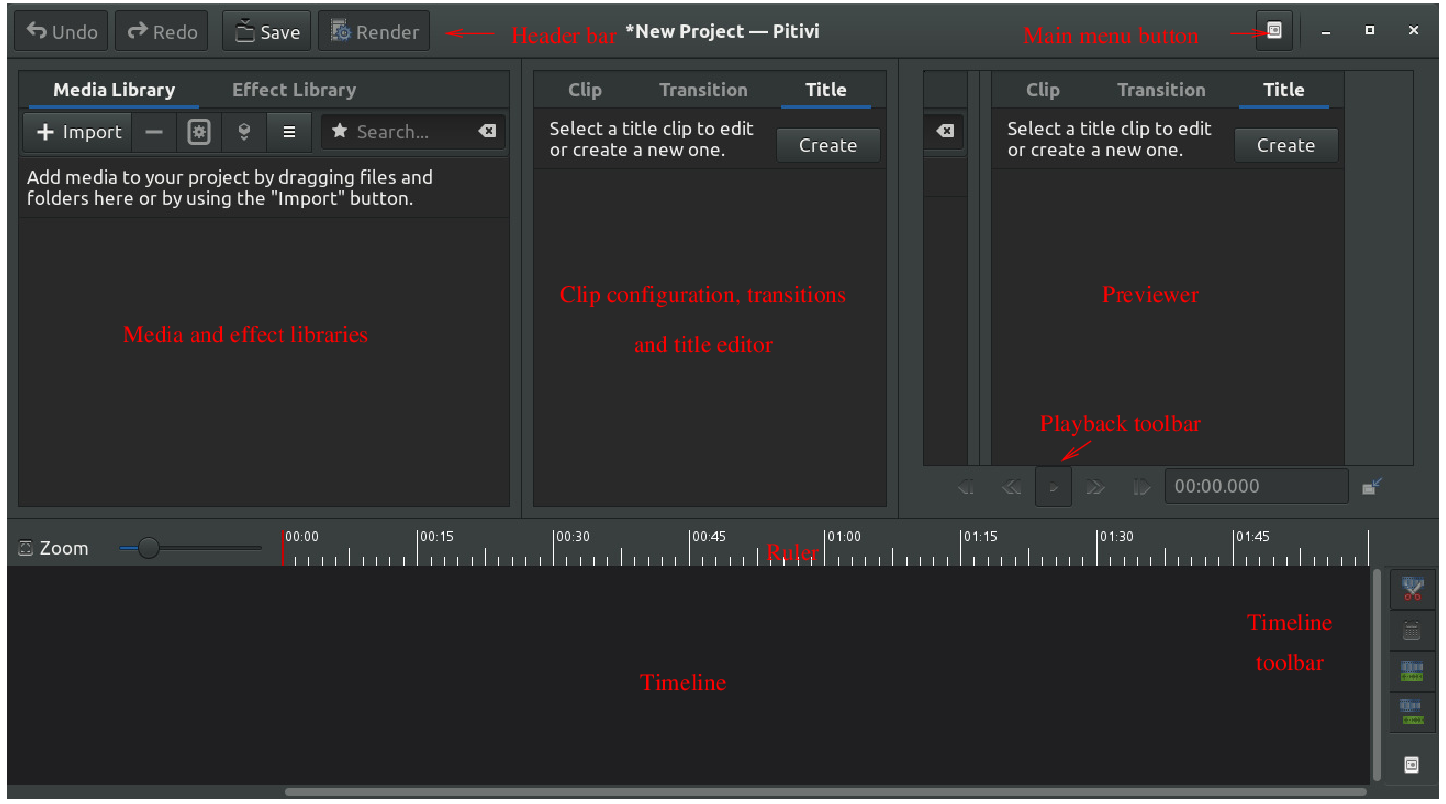
\includegraphics{main-window}
\end{center}

\begin{enumerate}
\item Header bar: Basic functions.
\item Ruler: A time scale.
\item Timeline: Contains the video layers.
\item Timeline toolbar: Timeline edition.
\item Playback toolbar: To control the playback.
\item Previewer: To view your results.
\item Media and effect libraries.
\item Clip configuration, transitions and title editor.
\end{enumerate}

%}}}


%}}}

\chapter{\href{http://www.pitivi.org/manual/importing.html}{Importing media}}
%{{{

\begin{verbatim}
wget http://techslides.com/demos/sample-videos/small.ogv
wget http://upload.wikimedia.org/wikipedia/commons/1/14/Xacti-AC8EX-Sample_video-001.ogg
\end{verbatim}

\begin{itemize}
\item To load a clip into Pitivi:
\begin{enumerate}
\item Use the file chooser dialog (\verb|Media Library -> Import|) or use drag and drop (from a file browser).
\item Clik on the button ``Insert the selected clips at the end of the timeline'' (this will concatenate the selected videos in the timeline).
\end{enumerate}
\end{itemize}

\begin{itemize}
\item Notice that clips can be placed/moved between layers (up and down). In this case, the playback will reproduce all videos in parallel (in the same canvas).
\end{itemize}

%}}}

\chapter{\href{http://www.pitivi.org/manual/movearoundtimeline.html}{Controlling the timeline}}
%{{{

\begin{enumerate}
\item [Activating the timeline toolbar]: Select a video clip with the mouse.
\item [Scrolling horizontally]: Use the mouse wheel anywhere over the
  timeline.
\item [Scrolling vertically]: Hold down the Shift key while using the
  mousewheel.
\item [Zooming in/out]: Holding the Ctrl key while using the
  mousewheel over the timeline.
\item [Change the position of the playhead]: Click on the ruler.
\item [Scrubbing]: Click on the ruler and move the mouse with the
  button still held down.
\end{enumerate}

%}}}

\chapter{\href{http://www.pitivi.org/manual/presets.html}{Presets}}
%{{{

\begin{center}
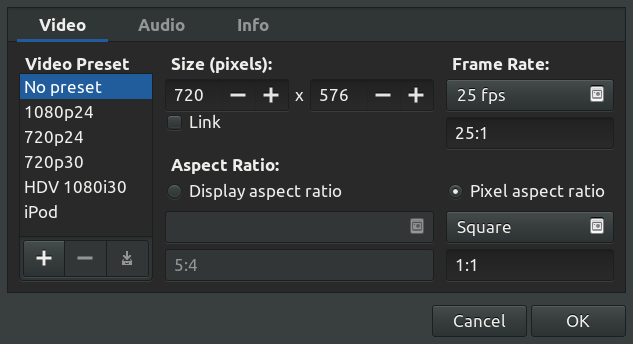
\includegraphics{presets-capture}
\end{center}

\begin{itemize}
\item Click on the Main menu button and select ``New project''.
\item Allows to define the rendering (output) settings.
\item Notice that new presets can be created.
\end{itemize}

%}}}

\chapter{\href{http://www.pitivi.org/manual/trimming.html}{Trimming (cut and paste)}}
%{{{

\section{Basic trimming}
%{{{

\begin{itemize}
\item Trimming is the act of changing the length of a clip by moving
  its beginning or end point in its timeline.
\item To perform a trimming do:
  \begin{enumerate}
  \item Move the mouse cursor over the edge of a clip and a trimming
    handle will appear.
  \item Drag the trimming handle in an appropriate direction to either
    reduce or increase the length of the clip.
  \end{enumerate}
\end{itemize}

%}}}

\section{Ripple editing}
%{{{

\begin{itemize}
\item Ripple editing is a variant of basic trimming which, in addition
  to trimming a clip, also moves the following clips.
  \item To perform a ripple edition do:
  \begin{enumerate}
  \item Place the mouse cursor on a trimming handle.
  \item Press and hold Shift.
  \item Drag the trimming handle.
  \end{enumerate}
\end{itemize}

%}}}

\section{Roll editing}
%{{{

\begin{itemize}
\item Roll editing is also a variant of basic trimming which, in addition
  to trimming a clip, trims the adjacent clips in a complementary way
  to prevent creating gaps.
\item To perform a ripple edition do:
  \begin{enumerate}
  \item Place the mouse cursor on a trimming handle between two adjacent clips.
  \item Press and hold Ctrl.
  \item Drag the trimming handle.
  \end{enumerate}
\end{itemize}

%}}}

%}}}

\chapter{\href{http://www.pitivi.org/manual/keyframecurves.html}{Keyframe curves}}
%{{{

\begin{itemize}
\item A keyframe is a frame (an image) of a video that does not depend
  on any other frame of the video when decoding.
\item The keyframe curve is a piecewise ``curve'' with vertices in the
  keyframes and that allows to change the opacity, effects, volumen,
  etc. of the clips on both, audio a video.
\item By default, all clips have an hidden fully-flat keyframe curve.
\item Most effects can be controlled with keyframes curves.
\item Keyframe (in yellow) curves appear when clicking on a layer. A vertice can be added by clicking on the keygrame curve.
\end{itemize}

%}}}

\chapter{\href{http://www.pitivi.org/manual/splitting.html}{Splitting}}
%{{{

\section{Split the current clip}
%{{{

\begin{itemize}
\item Divides the selected clip into two adjacent clips. Notice that
  if no clips are selected, all the clips under the playhead will be
  split.
\item To split a single clip:
\begin{enumerate}
\item Click on the clip.
\item Reposition the playhead (if needed).
\item Click on the Split button on the timeline toolbar or press S.
\end{enumerate}
\end{itemize}

%}}}

\section{Split all clips at the same time}
%{{{

\begin{itemize}
\item To split all the clips across the all layers:
  \begin{enumerate}
  \item Click on a blank area of the timeline (this will deselect all
    selected clips, if any).
  \item Reposition the playhead (the vertical red line of the timeline), if needed.
  \item Click on the Split button on the timeline toolbar or press S.
  \end{enumerate}
\end{itemize}

%}}}

\section{Split multiple clips}
%{{{

\begin{itemize}
\item To split multiple selected clips:
  \begin{enumerate}
  \item Position the playhead where you want to split.
  \item Add or remove clips to the selection with the Ctrl modifier
    key. This will not affect the playhead's position.
  \item Click on the Split button on the timeline toolbar or press S.
  \end{enumerate}
\end{itemize}

%}}}

%}}}

\chapter{\href{http://www.pitivi.org/manual/transitions.html}{Transitions}}
%{{{

\section{Fade-in/out}
%{{{

\begin{itemize}
\item Use the keyframe curve. You need to create for the fade-in an uphill slope and viceversa.
\end{itemize}

%}}}

\section{Crossfading (not implemented)}
%{{{

\begin{itemize}
\item To do a crossfade between two clips on the same layer, simply
  drag one of the clips onto the other so that it overlaps. By
  default, a linear transition will be created. A loop mode is also
  available.
\end{itemize}

%}}}

%}}}

\chapter{\href{http://www.pitivi.org/manual/effects.html}{Effects}}
%{{{

\begin{itemize}
\item Click on \verb|Effect library|.
\item Available effects depend on the software installed on your
  computer. If you don't see anything (or only a handful of effects)
  in the effect library, make sure that the gnome-video-effects
  package is installed on your system. Alternatively, you can look for
  packages containing GStreamer or frei0r effect plugins that are
  available in the repositories of your distribution.
\end{itemize}

\section{\href{http://www.pitivi.org/manual/usingeffects.html}{Adding (applying) effects}}
%{{{

\begin{enumerate}
\item Select an existing clip on the timeline.
\item Choose an effect in the effect library.
\item Drag the chosen effect into the
  \verb|middle pane -> Clip configuration -> Effects|.
\end{enumerate}

%}}}

\section{Removing effects}
%{{{

\begin{enumerate}
\item Select an existing clip on the timeline.
\item Select the effect from the
  \verb|middle pane -> Clip configuration -> Effects|.
\item Click the Remove effect button.
\end{enumerate}

%}}}

\section{Toggling effects}
%{{{

\begin{itemize}
\item If you want to temporarily disable an effect (to compare with
  and without the effect, or for performance reasons), click the
  corresponding \verb|Active| checkbox in the
  \verb|middle pane -> Clip configuration -> Effects|.
\end{itemize}

%}}}

%}}}
